\section{Przykładowa lista}
\suppressfloats[t]
\begin{itemize}
  \item \textit{yyy} - ola ma psa
  \item \textit{zzz} - ela ma misia
  \item \textit{xxx} - ala ma kota
\end{itemize}



\section{Przykładowa tabela}

\begin{tabularx}{\textwidth}{X|l|X}
\hline
\textbf{A} & \textbf{B} & \textbf{Ce} \\ \hline
xxx         & xxx         & xxx          \\ \hline
yyy          &yyy         & yyy            \\ \hline
\end{tabularx}

\section{Przykładowy rysunek}

\begin{figure}[!tb]
    \centering
    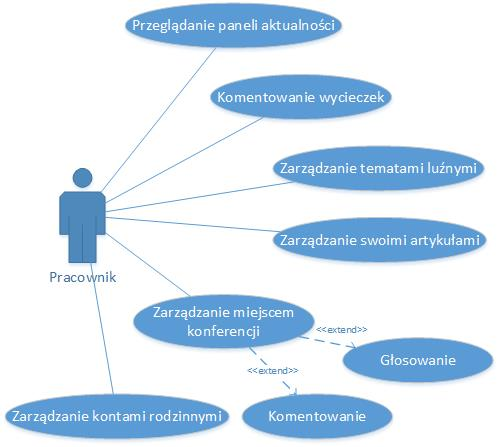
\includegraphics{pracownik.jpg}
    \caption{Przykładowy rysunek.}
    \label{fig:pracownik}
\end{figure}

\section{}